\subsection{Model}\label{sec:model}
\begin{definition}[Weighted graph]\label{def:graph}
A weighted graph is a triple $G=(V,E,w)$ with $w:E\to\mathbb{R}_{\ge 0}$.
\end{definition}
\begin{figure}[H]
\centering
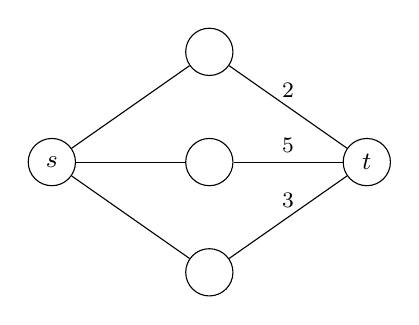
\begin{tikzpicture}[v/.style={circle,draw,minimum size=6mm,inner sep=0pt,font=\small}]
  \node[v] (s) at (0,0) {$s$};
  \node[v] (t) at (4,0) {$t$};
  \foreach \y/\i/\w in {1.4/1/2,0/2/5,-1.4/3/3}{
     \node[v] (m\i) at (2,\y) {};
     \draw (s)--(m\i); \draw (m\i)--node[above,font=\footnotesize]{\w}(t);
  }
\end{tikzpicture}
\caption{A small weighted graph with three routes from $s$ to $t$.}\label{fig:graph}
\end{figure}
A numbered equation and a two-line aligned one:
\begin{equation}\label{eq:path}
  d(s,t) \;=\; \min_{P}\ \sum_{e\in P} w(e)
\end{equation}
\begin{align}
  T_{\text{merge}}(n) &= 2\,T_{\text{merge}}(n/2) + n, \label{eq:merge}\\
  T_{\text{merge}}(n) &= O(n\log n). \nonumber
\end{align}
